%===================================================================================================
% INCLUDES

\documentclass[12pt,a4paper,oneside]{article}	% Fonttikoko ja dokumenttityyppi
\usepackage[a4paper,bindingoffset=0.2in,%
            left=0.75in,right=0.75in,top=0.6in,bottom=0.6in,%
            footskip=.25in]{geometry}
\usepackage{float}
%\usepackage[finnish]{babel}			% Kieli- ja tavutuspaketit
\usepackage[utf8]{inputenc}   			% merkistökoodaus, jos käytetään UTF8:a
\frenchspacing
\usepackage[babel]{csquotes}
\usepackage[backend=bibtex, sorting=none, style=nature]{biblatex} 	% BibLatex > NatBib
%\usepackage{hyphenat}  				% Tavutuksen viilaamiseen liittyvä (hyphenpenalty,...)
\usepackage{amsmath}					% Matematiikkaa
\usepackage{empheq}						% Matematiikkaa
\usepackage{url}
\usepackage{graphicx}
\usepackage{subfigure}
\usepackage{url}						% use \url{}. Prefix with \protect to use in captions and labels
\usepackage{gensymb}					% Degree symbol with \degree
\usepackage{amssymb}
\usepackage{caption}					% Mahdollistaa captionit ilman numerointia
\usepackage{sectsty}
\usepackage{hyperref}
\usepackage{datetime}

% CUSTOM COMMAND DEFINITIONS
%\renewcommand{\vec}[1]{\mathbf{#1}}				% vectors with bold
\newcommand{\+}[1]{\ensuremath{\mathbf{#1}}}		% Produce bold and upright vectors and matrices with \+
\newcommand{\eq}[2]{\mathrel{\operatorname*{=}_{#1}^{#2}}}
\newcommand{\HRule}{\rule{\linewidth}{0.5mm}} % Defines a new command for the horizontal lines, change thickness here
\sectionfont{\fontsize{15}{15}\selectfont}

% COMMANDS
\bibliography{bibliography}

%----------------------------------------------------------------------------------------
%	TITLE PAGE
%----------------------------------------------------------------------------------------
\begin{document}

%----------------------------------------------------------------------------------------
%	BRIEFLY
%----------------------------------------------------------------------------------------
\begin{flushleft}
\Large\textbf{Summer Student Project: Crystal Structure Map}\\
\vspace{0.2cm}
\large By: Lauri Himanen\\
\large Date: \today\\
\end{flushleft}

%----------------------------------------------------------------------------------------
%	BACKGROUND
%----------------------------------------------------------------------------------------
\section*{Introduction}
When working with large datasets of heterogeneous crystal structures, understanding how the different structures are distributed in the structural and chemical space is an important task. With the advent of large material repositories and datasets, this task is becoming vital in order to effectively visualize structures in large repositories e.g. for search purposes or in order to analyze the composition of a dataset used in machine learning.

Crystal structures are often described through their symmetry properties, such as space group number, bravais lattice, crystal lattice or Wyckoff positions. Such a mapping helps, but can be misleading because the symmetry properties are discontinuous with respect to small changes in the coordinates of atoms in the unit cell, and the results are often difficult to interpret for the non-expert.

In this project we will investigate an alternative approach, where the structural and chemical features are represented as a feature vector that is projected to an easily visualizable lower dimensional space by using data clustering or projection algorithms which are a part of unsupervised machine learning methods.

%----------------------------------------------------------------------------------------
%	Objectives
%----------------------------------------------------------------------------------------
\section*{Objectives and methods}

The final objective of the project is to create a method for mapping and visualizing large datasets of crystal structures. In order to test the ideas we have prepared a set of roughly 30 000 crystal structures from the AFLOW database\cite{aflow1}. The project is divided into three key topics: choosing the descriptor, clustering and projection, and presentation. Depending on the time and your interests, you can choose how you want to divide your time on these tasks.
\\\\
\noindent\textbf{Choosing the descriptor}\\
In order for clustering methods to work, we need to define how crystal structures are presented to the algorithm. Typically such structures are represented by using a unit cell, atom positions and chemical elements of atoms. Such an input feature is however not directly suitable for clustering or machine learning in general. There are multiple reasons for this, including the fact than an XYZ-coordinate representation is not invariant to rotations or translations. In order to address this problem, multiple feature transformation have been proposed\cite{cm, mbtr, soap, voronoi, acsf}. These transformations are here rererred to as descriptors. We will start by using the many-body tensor representation (MBTR) \cite{mbtr}, but can investigate other models as needed. MBTR captures the crystal structure as a ``spectrum'' of atomic distances and angles, as illustrated in image \ref{fig:mbtr}.
\begin{figure}[h!]
  \centering
  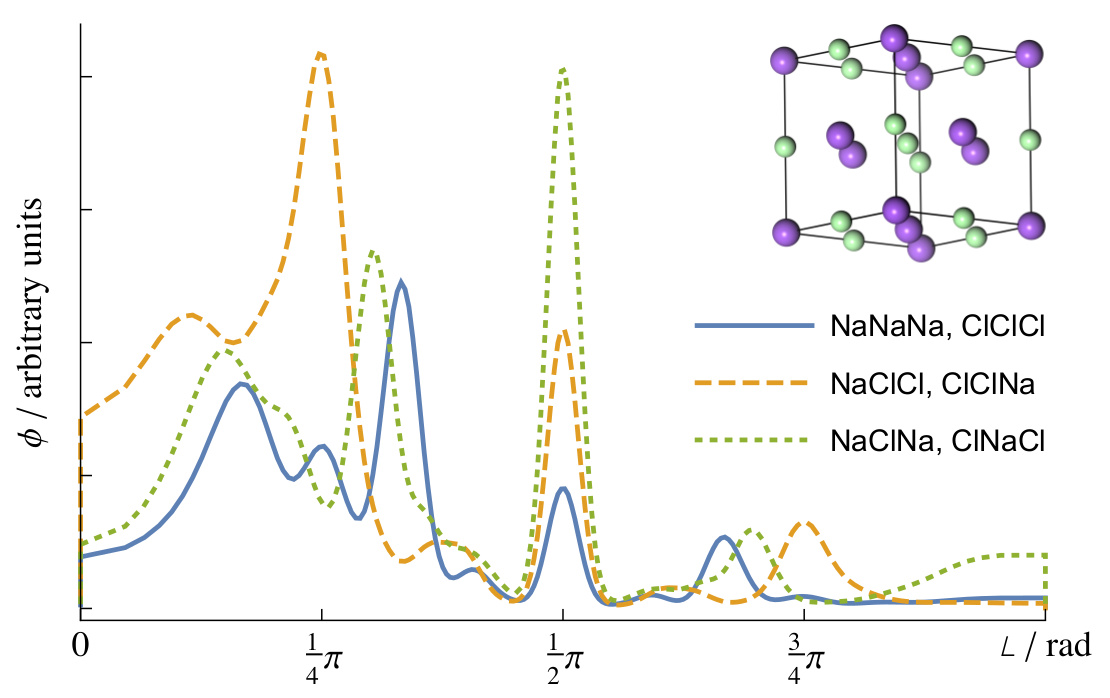
\includegraphics[width=7cm]{mbtr.jpg}
  \caption{The MBTR spectrum for angles in a sodium-chloride crystal.}
  \label{fig:mbtr}
\end{figure}
\\\\
\noindent\textbf{Clustering and projection}\\
The chosen descriptor effectively captures the structural features of a crystal in a n-dimensional space, which cannot be visualized or understood directly. In order to make sense of these feature vectors, we will use an unsupervised machine learning method that can be used to transform the data into a 2D or 3D.

A simple approach is to define an euclidean metric in the descriptor space, and calculate distances between crystal as the euclidean distance between two descriptor vectors. This approach can be used together with clustering algorithms such as DBSCAN\cite{dbscan} and graph layout algorithms to produce a map of the crystal space.

An alternative approach is to perform a projection of the n-dimensional space into a lower dimensional one that can be more easily visualized. There are multiple approaches for doing such tasks, including PCA\cite{pca}, t-SNE\cite{tsne} and UMAP\cite{umap}. An example of t-SNE clustering of hand-writtend digits is given in figure \ref{fig:tsne}.

There is a very nice introduction to different visualization methods given here: \url{http://colah.github.io/posts/2014-10-Visualizing-MNIST/}.
\begin{figure}[h!]
  \centering
  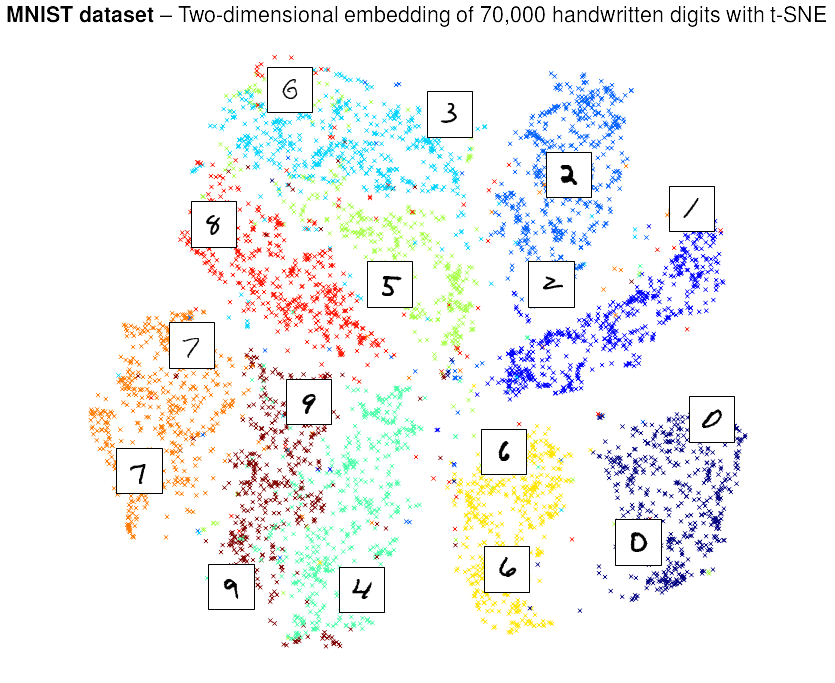
\includegraphics[width=8cm]{tsne.png}
  \caption{Illustration of t-SNEs capability to reduce multidimensional input into meaningful categories in a lower-dimensional space. The input data is an MNIST dataset of hand-written digits as 28x28 grayscale images, which has been clustered into groups representing different digits. Original image from \url{http://alexanderfabisch.github.io/t-sne-in-scikit-learn.html}}
  \label{fig:tsne}
\end{figure}
\\\\
\noindent\textbf{Presentation}\\
In order to make sense of the dataset we need to present the results in 2D or 3D space. For this purpose we could create an interactive web-based presentation that allows one to visualize the data in a browser. To make the interpretation easy, we can provide a visualization of the individual crystals directly in this tool, and encode other crystal properties (energy, band gap, symmetry properties, etc.) as colours or sizes of the nodes in the visualization.

%----------------------------------------------------------------------------------------
%	Getting started
%----------------------------------------------------------------------------------------
\section*{Getting started}

\begin{itemize}
  \item Understanding what unsupervised machine learning is, and how it differs from supervised learning. Depending on your interest also getting to know other machine learning techniques.
    \begin{itemize}
      \item Machine learning course in Coursera, by Andrew Ng: \url{https://www.coursera.org/learn/machine-learning}.
      \item \url{https://en.wikipedia.org/wiki/Machine_learning}.
    \end{itemize}
  \item Reading about dimensionality reduction techniques for visualization:
  \begin{itemize}
    \item Visualizing MNIST: An Exploration of Dimensionality Reduction: \url{http://colah.github.io/posts/2014-10-Visualizing-MNIST/}
  \end{itemize}
  \item Reviewing basic theory behind crystal structures:
    \begin{itemize}
      \item E.g. Girolami, Gregory S. (2016). X-Ray Crystallography. University Science Books, Section 1 \url{https://app.knovel.com/web/toc.v/cid:kpXRC00001/viewerType:toc/root_slug:x-ray-crystallography/url_slug:x-ray-crystallography}  (or any basic book on crystallography).
    \end{itemize}
  \item Reading about the rational and techniques behing descriptors:
    \begin{itemize}
      \item E.g. Many-Body Tensor Representation for Machine Learning of Atomistic Systems \url{https://arxiv.org/abs/1704.06439}
    \end{itemize}
\end{itemize}

%----------------------------------------------------------------------------------------
%	REFERENCES
%----------------------------------------------------------------------------------------
\renewcommand*{\bibfont}{\scriptsize}
\printbibliography


\end{document}